\documentclass{beamer}

\usepackage{beamerthemesplit}

\usetheme{Berkeley}
\useinnertheme{circles}
\usecolortheme{seagull}

\title[Stereo vision]{Stereo Vision using the OpenCV library \\ A glance}
\author[Dr\"oppelmann \and Hueting \and Latour \and \\Van der Veen]{Sebastian Dr\"oppelmann \\ Moos Hueting \\ Sander Latour \\ Martijn van der Veen}
\institute{University of Amsterdam}
\date{June 2010}
\subject{Computer vision}

\begin{document}

\graphicspath{{./images/}}

\frame
{
  \titlepage
}

\section{Recap}

\frame
{
 \frametitle{Goal}
 \begin{block}{Goal}
   Generating a disparity depth map of the environment using stereo vision.
 \end{block}
}

\frame{
 \frametitle{Intended end-result}
 \begin{figure}
   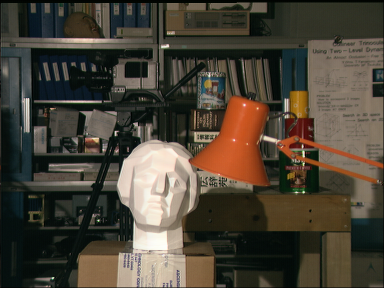
\includegraphics[width=0.3\textwidth]{exampleleft}
   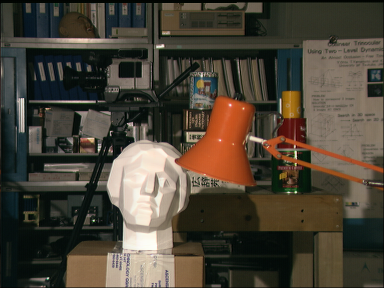
\includegraphics[width=0.3\textwidth]{exampleright}
   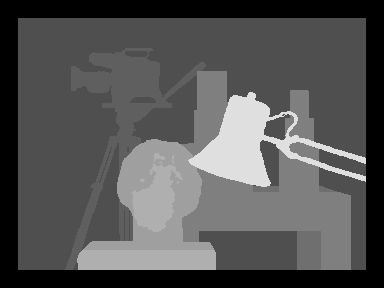
\includegraphics[width=0.3\textwidth]{exampledepth}
   \caption{Stereo images with disparity depth map}
 \end{figure}
}

\section{Demonstration}

\frame{
  \frametitle{Calibration}
  \begin{itemize}
    \item Retrieve spatial relation between cameras
    \item Demo
  \end{itemize}
}

\frame{
  \frametitle{Rectification}
  \begin{itemize}
    \item Calculate rectification parameters
    \item Reusable
  \end{itemize}
}

\frame{
  \frametitle{Stereo correspondence}
  \begin{itemize}
    \item Multiple methods
  \end{itemize}
}

\end{document}
